\chapter{\IfLanguageName{dutch}{Analyse van de cijfers}{Analysis of the figures}}%
\label{ch:analyse}

Allereerst werden de deelnemers van het onderzoek online bevraagd via een vragenlijst. Daarbij werd vooral gepeild naar:
\begin{itemize}
    \item hoe tevreden deelnemers zijn over hun hoeveelheid beweging,
    \item hoeveel ze bewegen,
    \item wat in hen de weg staat om meer te bewegen,
    \item welk gevoel gamification teweegbrengt,
    \item wat belangrijk is voor hen in een sportapplicatie.
\end{itemize}

Daarna is de POC, zoals beschreven in hoofdstuk \ref{ch:proofofconcept}, in gebruik genomen door diezelfde mensen. Tenslotte is nogmaals een vragenlijst uitgestuurd om eventuele veranderingen of evoluties op te merken en te analyseren.

De éénentwintig bevraagde mensen zijn allen werkzaam in een sedentaire job. 42.9\% van de respondenten zijn tussen de 18 en 25 jaar oud, 42.9\% tussen de 25 en 35 jaar oud en de overige 14.3\% zijn tussen de 35 en 45 jaar oud (figuur \ref{fig:leeftijd}). Deze bachelorproef kan daarom geen conclusies trekken over mensen die zich buiten deze leeftijdsgroepen bevinden. Gezien de omvang van de steekproef, kan deze bachelorproef  suggesties doen die aanzet geven naar verder onderzoek.

\begin{figure}
    \caption[Verdeling van de leeftijd van deelnemers]{Verdeling van de leeftijd van deelnemers.}
    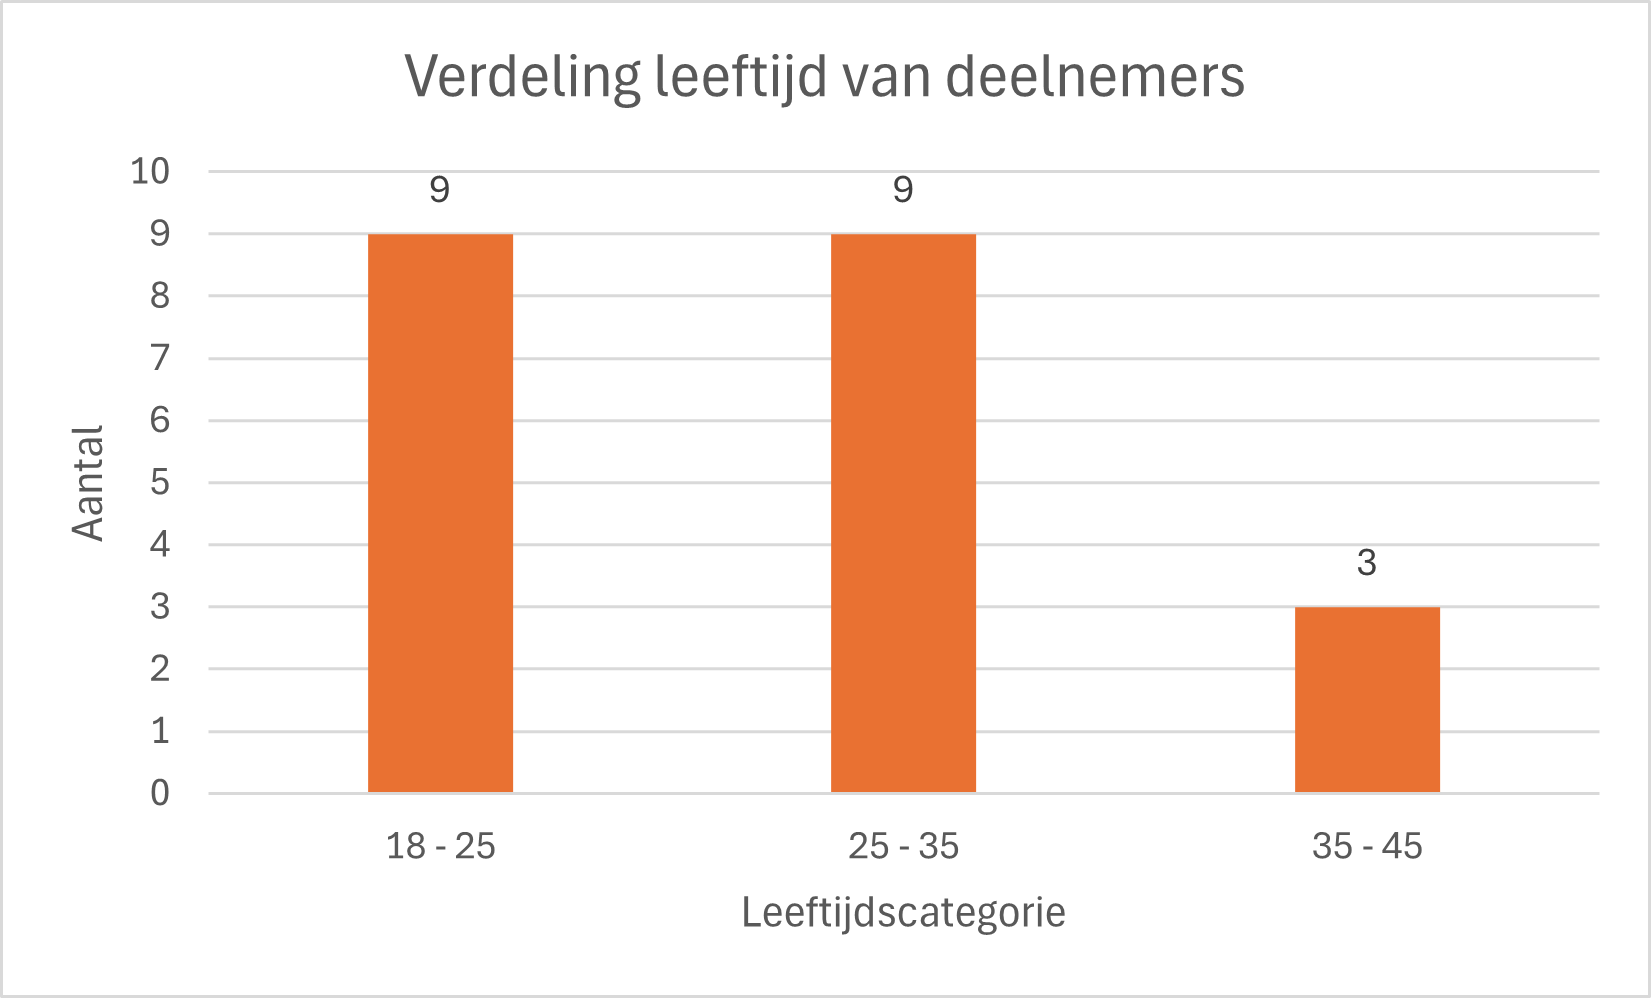
\includegraphics[width=1\textwidth]{LeeftijdVerdeling}
    \label{fig:leeftijd}
\end{figure}

\section{Resultaten voor gebruik van ``Move-it!''}

\subsection{Beweging}
Slechts 33.3\% van de bevraagde personen is tevreden met diens hoeveelheid dagelijkse beweging (zie figuur \ref{fig:dagelijkseBeweging}).

\begin{figure}
    \caption[In welke mate vindt u van uzelf dat u dagelijks voldoende beweegt?]{In welke mate vindt u van uzelf dat u dagelijks voldoende beweegt (op een schaal van 1 tot en met 5)?}
    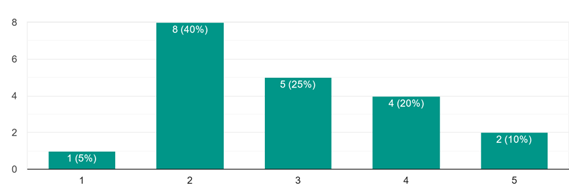
\includegraphics[width=1\textwidth]{DailyMovement}
    \label{fig:dagelijkseBeweging}
\end{figure}

Volgens de WHO moeten volwassenen tussen de 18 en 64 jaar oud wekelijks ongeveer 150 à 300 minuten met gemiddelde intensiteit sporten \autocite{Bull2020}.

Uit deze vragenlijst is gebleken dat 47.5\% van de 18 à 45 jarigen dit voorgeschreven aantal niet halen (figuur \ref{fig:gemiddeldSporten}). Dit wil zeggen dat 52.5\% van de mensen dit aangeraden aantal behaalt. 19.1\% van hen sport zelfs meer dan 5 uur per week met gemiddelde intensiteit. Het is binnen dit onderzoek niet mogelijk te achterhalen of een deel van deze 52.5\% dezelfde mensen zijn als de 33.3\% die tevreden zijn met hun hoeveelheid dagelijkse beweging. Het is echter wel een interessante piste die vraagt om verder onderzoek.

De WHO stelt dat volwassenen van diezelfde leeftijdsgroep ongeveer 75 à 150 minuten met hoge intensiteit moeten sporten \autocite{Bull2020}.
52.4\% van de respondenten behaalt dit doel en 33.5\% van hen doet zelfs meer dan de aangeraden 150 minuten (figuur \ref{fig:intensiefSporten}).

\begin{figure}[h]
    \caption[Hoeveel sport u wekelijks met gemiddelde intensiteit?]{Hoeveel sport u wekelijks met gemiddelde intensiteit?}
    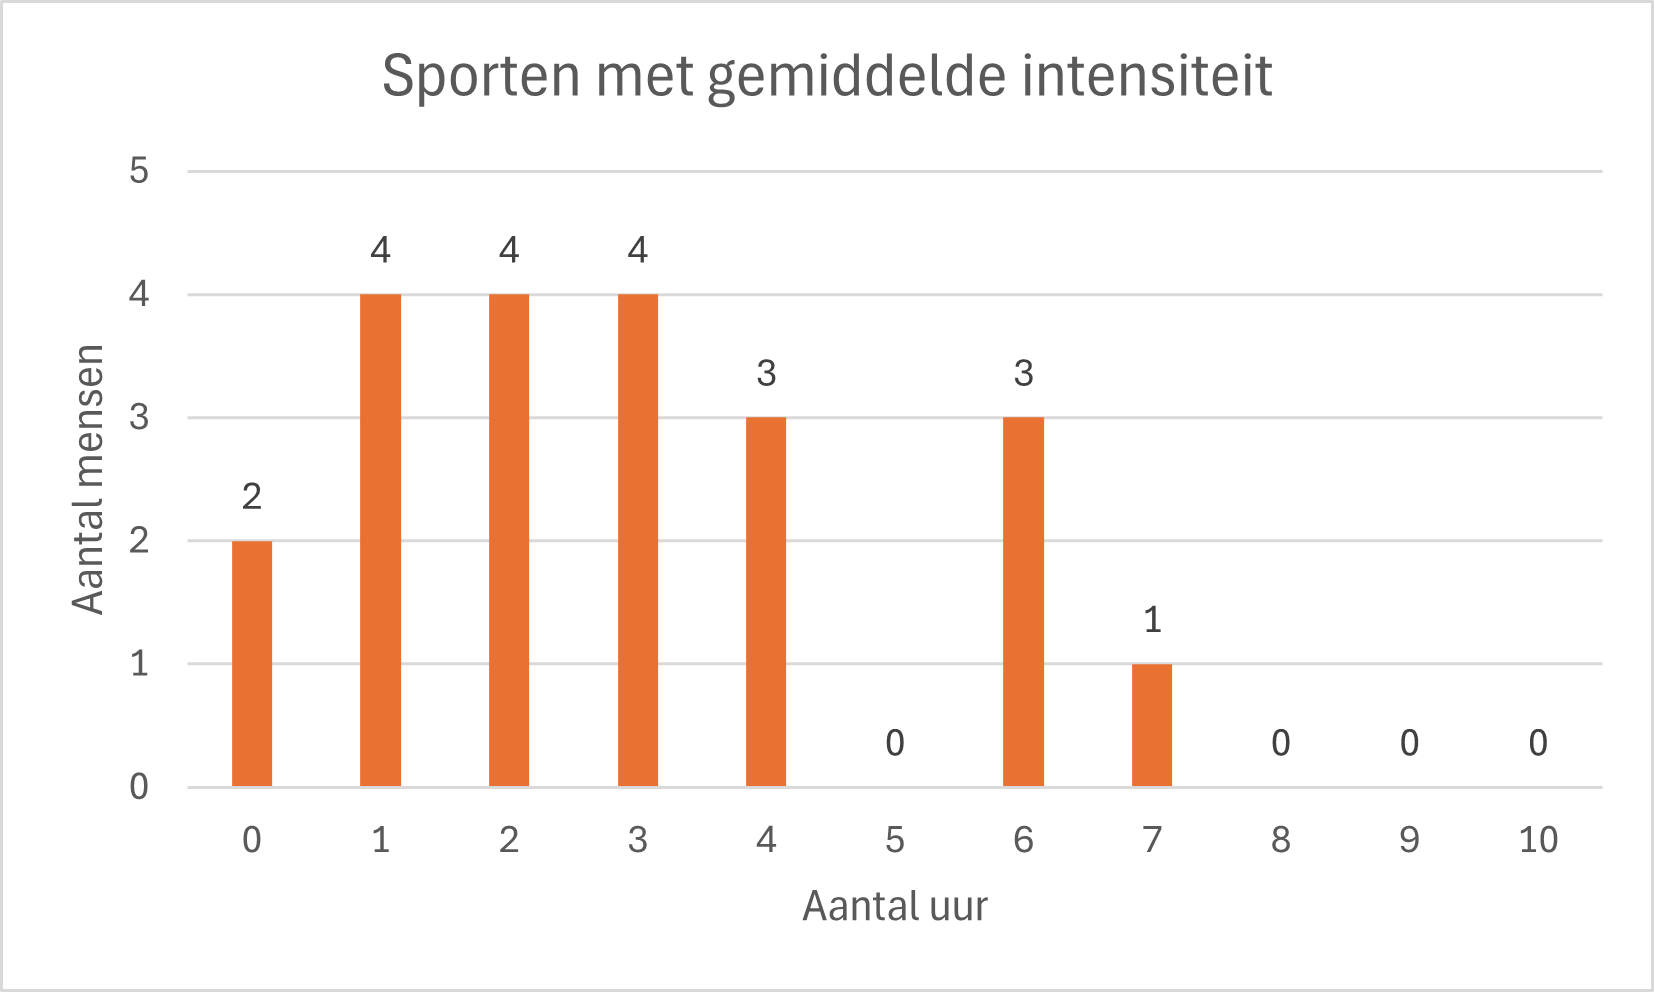
\includegraphics[width=1\textwidth]{SportenGemiddeld}
    \label{fig:gemiddeldSporten}
\end{figure}

\begin{figure}[h]
    \caption[Hoeveel sport u wekelijks met hoge intensiteit?]{Hoeveel sport u wekelijks met hoge intensiteit?}
    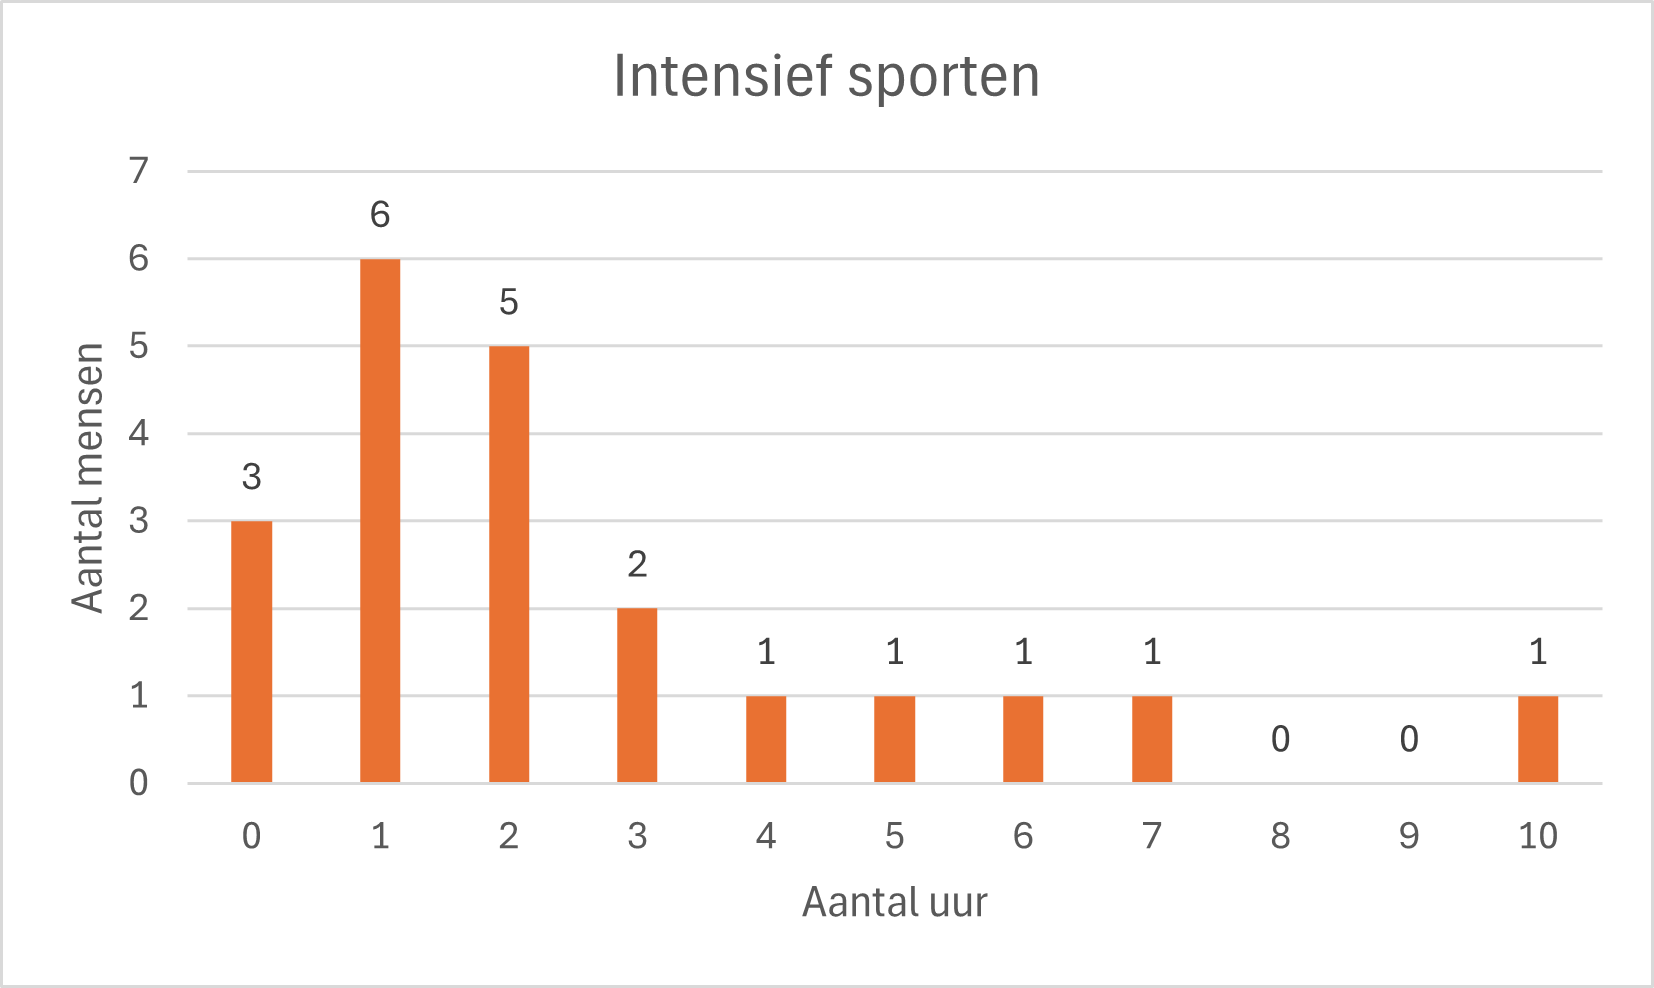
\includegraphics[width=1\textwidth]{SportenIntensief}
    \label{fig:intensiefSporten}
\end{figure}

\subsection{Motivatie}

Slechts vier van de éénentwintig mensen zijn tevreden met de hoeveelheid sport die ze op dit moment beoefenen. Dit wil zeggen dat ruim 81\% niet tevreden is en liever meer zou sporten of bewegen (zie figuur \ref{fig:meerBewegen}).

Het grootste probleem voor mensen om meer te sporten, is tijd vinden. Daarnaast staan ook motivatie en wederkerende blessures in de weg. Een minderheid vindt ook geen plezier in het sporten (zie figuur \ref{fig:waarom}).

\begin{figure}[h]
    \caption[Zou u liever meer sporten dan u op dit moment doet?]{Zou u liever meer sporten dan u op dit moment doet?}
    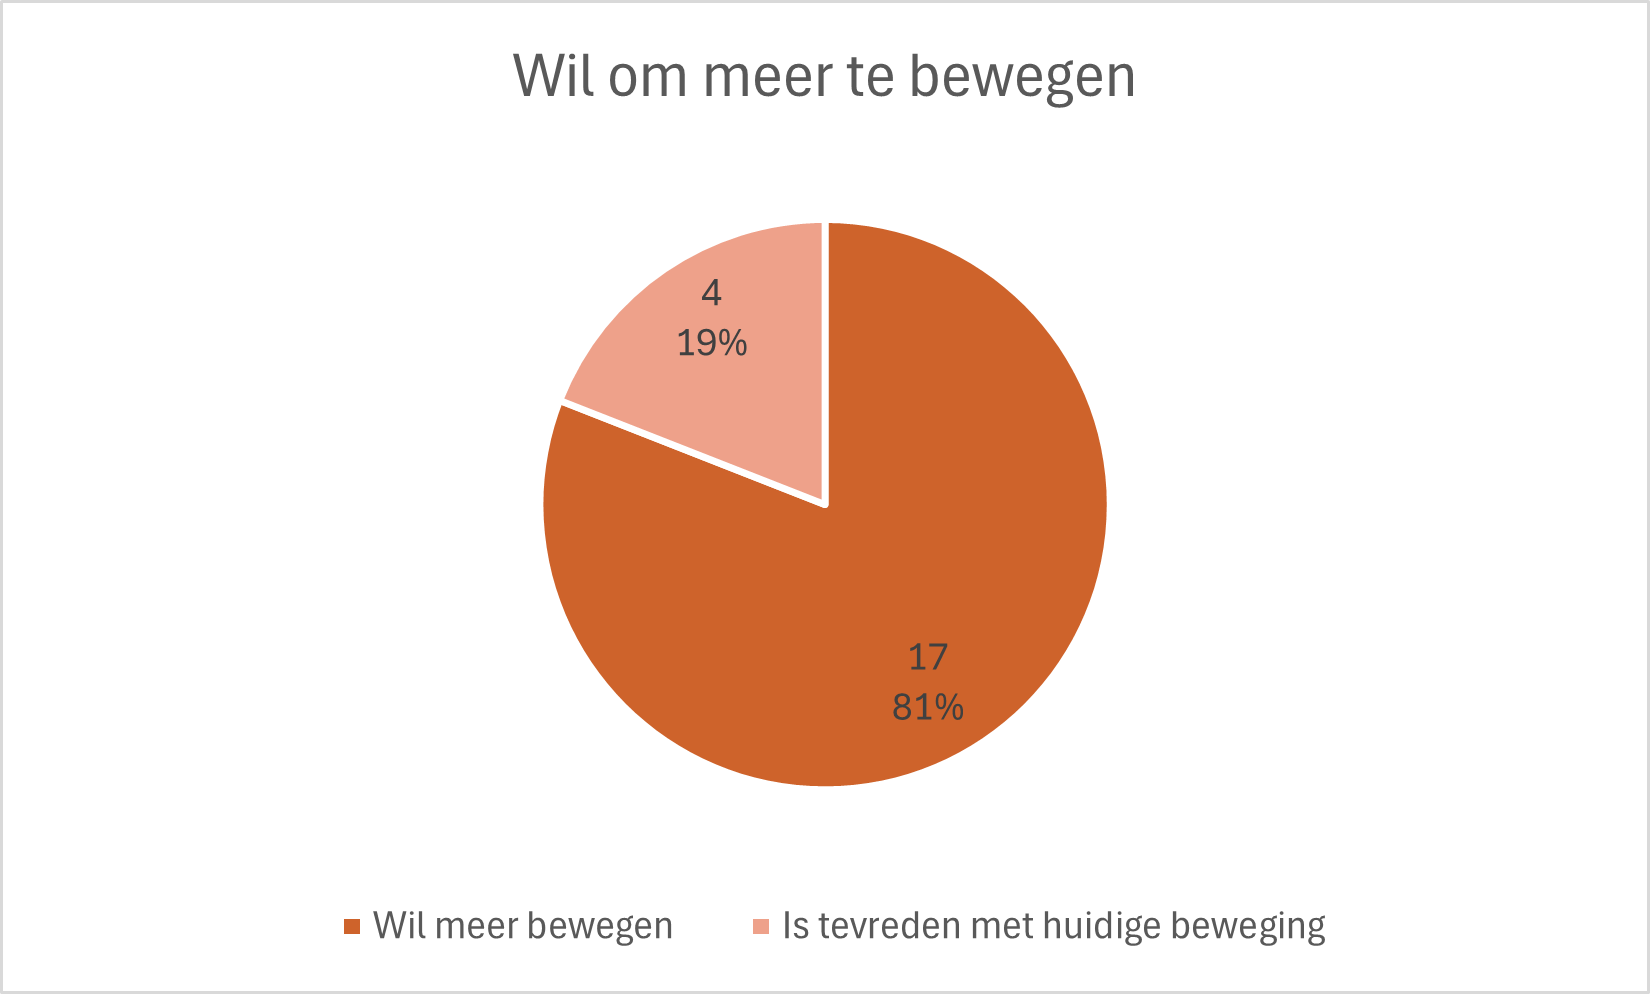
\includegraphics[width=1\textwidth]{MeerSporten}
    \label{fig:meerBewegen}
\end{figure}

\begin{figure}[h]
    \caption[Wat houdt u op dit moment tegen om meer te sporten?]{Wat houdt u op dit moment tegen om meer te sporten?}
    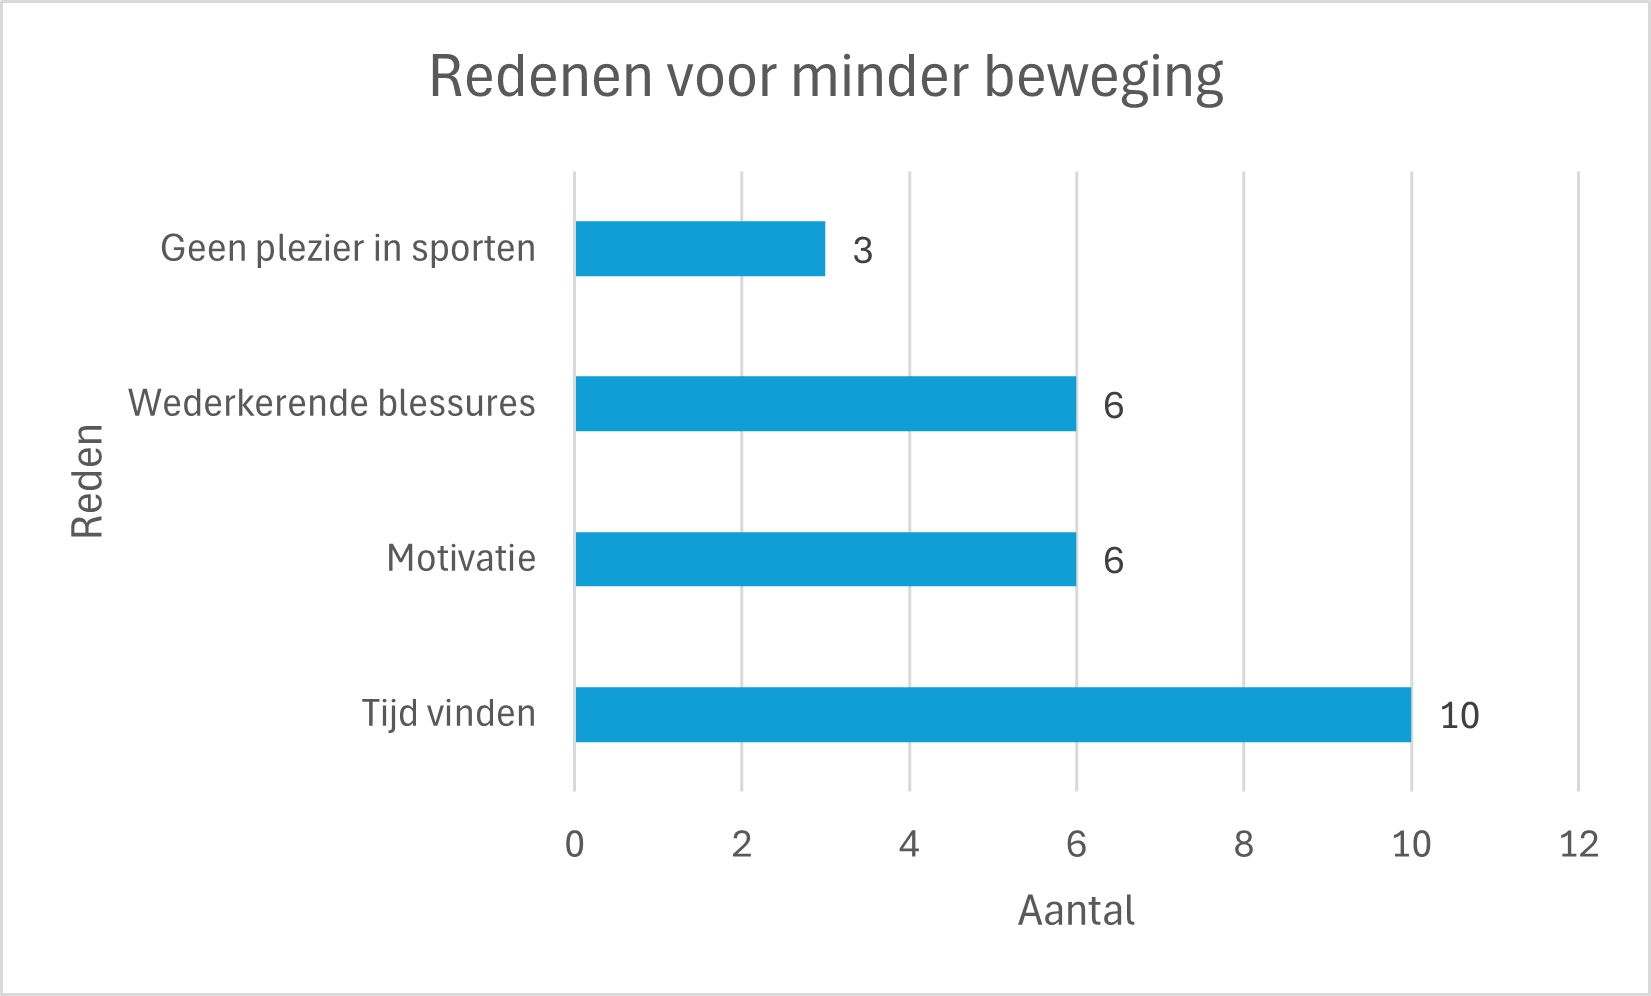
\includegraphics[width=1\textwidth]{Waarom}
    \label{fig:waarom}
\end{figure}

\subsection{Gamification}

Op vlak van het type gamification in het algemeen, is er een duidelijke voorkeur: 76.2\% van de respondenten verkiest een focus op het zien van persoonlijke vooruitgang. In de applicatie werd deze geïmplementeerd in de vorm van twee grafieken, zoals te zien is op figuur \ref{fig:graphs}.

Dit kan ook teruggevonden worden in wat belangrijk gevonden wordt in een sportapplicatie. 95.2\% vindt het meten van deze persoonlijke vooruitgang, binnen een specifieke sportcontext, namelijk belangrijk en 71.4\% vindt ook technische gegevens zien over de activiteit een meerwaarde.

\subsubsection{Sociale aspecten}

Het valt ook op dat sociale interacties, zoals bijvoorbeeld likes, comments en volgers, net als storend ervaren worden door 47.6\%. Dit is tegenstrijdig met wat de literatuur stelt. Daar wordt beschreven hoe gebruikers enerzijds sociale feedback, en anderzijds sociale invloed nodig hebben (zie subsectie \ref{ssec:sociale_aspecen}).Een mogelijke verklaring hiervoor zou kunnen zijn dat dit wordt ervaren als sociale druk, wat de deelnemers angstgevoelens kan bezorgen, uit vrees om niet aan de verwachtingen te voldoen \autocite{Jong2010}. Dit onderzoek heeft ervoor gekozen om geen gebruik te maken van sociale interacties en gaat daarom niet op zoek naar een bevestiging of ontkrachting van deze potentiële achterliggende reden.

\subsubsection{Psychologische aspecten: motivatie}

Het is daarnaast ook tegenstrijdig dat 38.1\% uitgedaagd en gemotiveerd wil worden door de applicatie, terwijl 42.9\% het storend vindt meldingen te ontvangen van een sportapplicatie. Dit wil zeggen dat gebruikers van deze applicatie op andere manieren dan gewoonlijk gemotiveerd willen worden.
De huidige meest voorkomende vorm van motivatie gebeurt namelijk door middel van pushmeldingen:
Strava motiveert bijvoorbeeld door notificaties te sturen wanneer iemand van je sociale kring een nieuwe activiteit post, je voorbijgestoken wordt in een klassement of wanneer je een doel bereikt.

\subsection{Meest gebruikte sportapplicaties}

Strava is de populairste sportapplicatie binnen deze steekproef: 85.7\% van de deelnemers geeft aan Strava te gebruiken. Daarna volgen Garmin Sports (28.6\%), Adidas Runtastic (19\%), Apple Workouts (19\%) en Nike Run Club (9.5\%). Niemand uit deze steekproef gebruikt Fitbit. Er zijn ook 2 personen die geen sportapplicaties gebruiken.

\section{Sportresultaten}

Op figuren \ref{fig:evolutie1}, \ref{fig:evolutie2}, \ref{fig:evolutie3}, \ref{fig:evolutie4}, \ref{fig:evolutie5}, \ref{fig:evolutie6}, \ref{fig:evolutie7} en \ref{fig:evolutie8} wordt de evolutie weergegeven van een deel van de deelnemers van dit onderzoek. Deze zijn uit de steekproef gekozen door de consistentie waarmee ze data hebben ingegeven. Van andere deelnemers is het minder waarschijnlijk dat de ingevoerde data een realistische representatie is. Het valt hierbij op dat vooral jongere mensen (van 22 tot en met 28 jaar) gemotiveerd waren om sportgegevens in te vullen. In de volgende sectie wordt besproken wat hier mogelijke oorzaken van kunnen zijn.

Bij vijf van de acht deelnemers, is er een stijging waarneembaar in de hoeveelheid dagelijkse beweging. Drie personen bleven met dezelfde intensiteit en frequentie bewegen. In het volgende deel van dit onderzoek wordt bevraagd of deze stijging al dan niet te maken heeft met de ingebruikname van het sportplatform.

\begin{figure}[htbp]
    \begin{minipage}[t]{0.48\linewidth} % adjust width as needed
        \centering
        \caption[Evolutie van de activiteit van een 27-jarige]{Evolutie van de activiteit ingegeven in ``Move-it!'' van een 27-jarige.}
        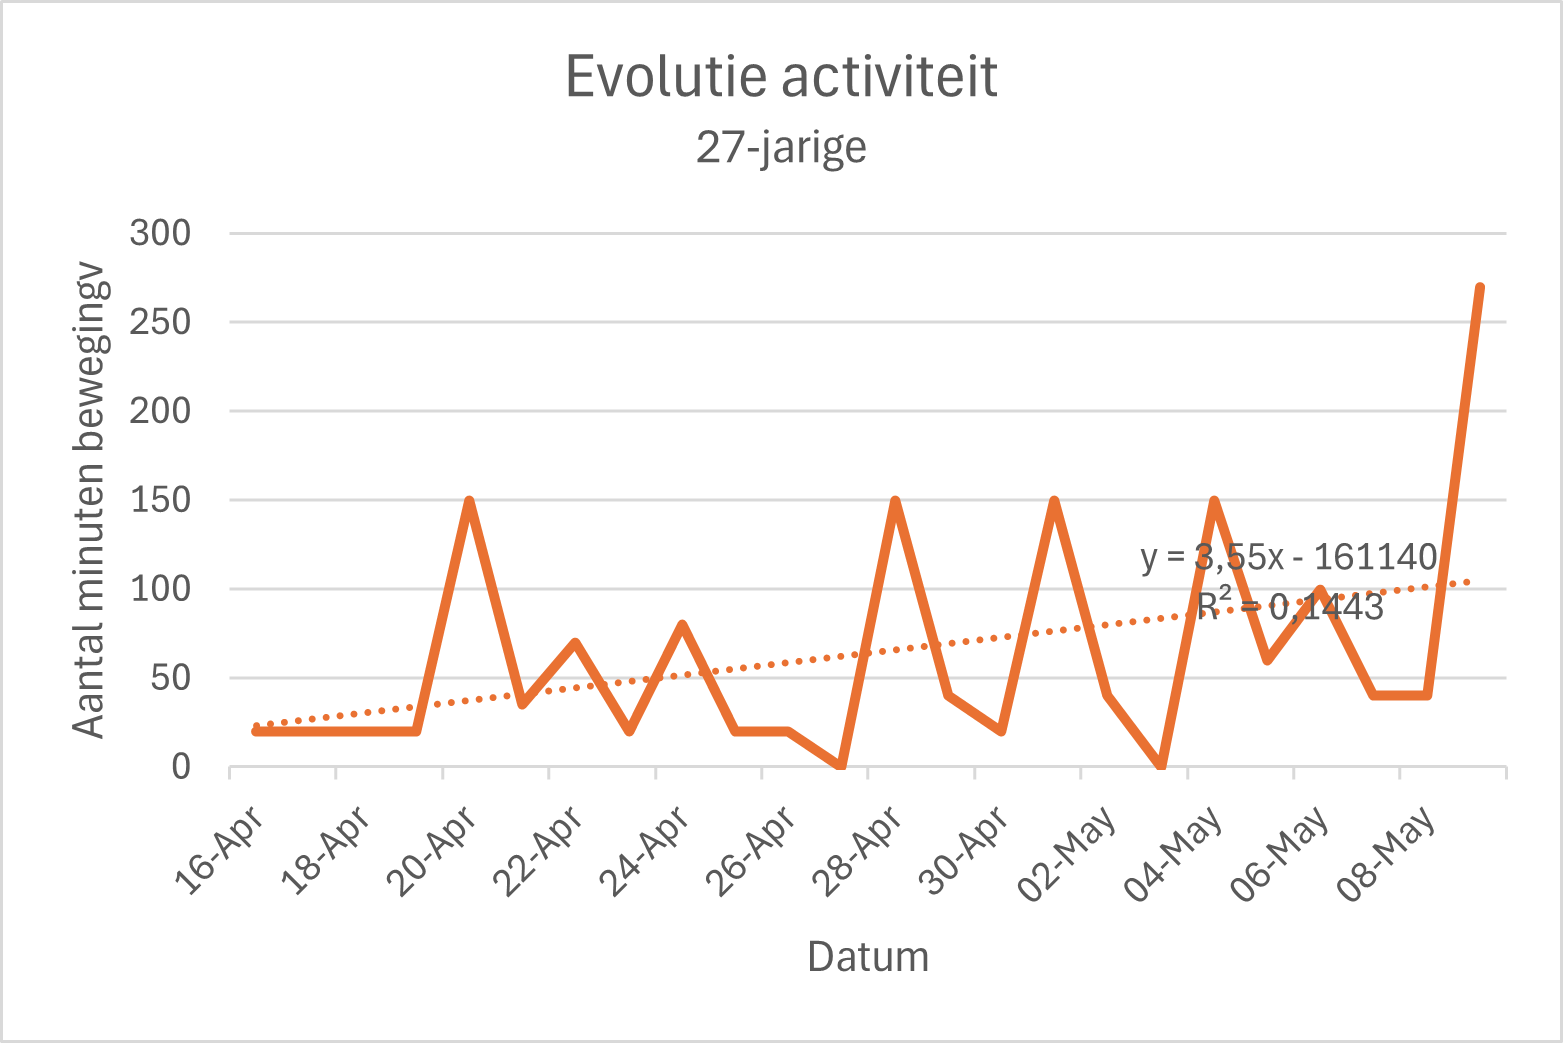
\includegraphics[width=1\textwidth]{GrafiekEvolutie1}
        \label{fig:evolutie1}
    \end{minipage}
    \hfill
    \begin{minipage}[t]{0.48\linewidth} % adjust width as needed
        \centering
        \caption[Evolutie van de activiteit van een 22-jarige]{Evolutie van de activiteit ingegeven in ``Move-it!'' van een 22-jarige.}
        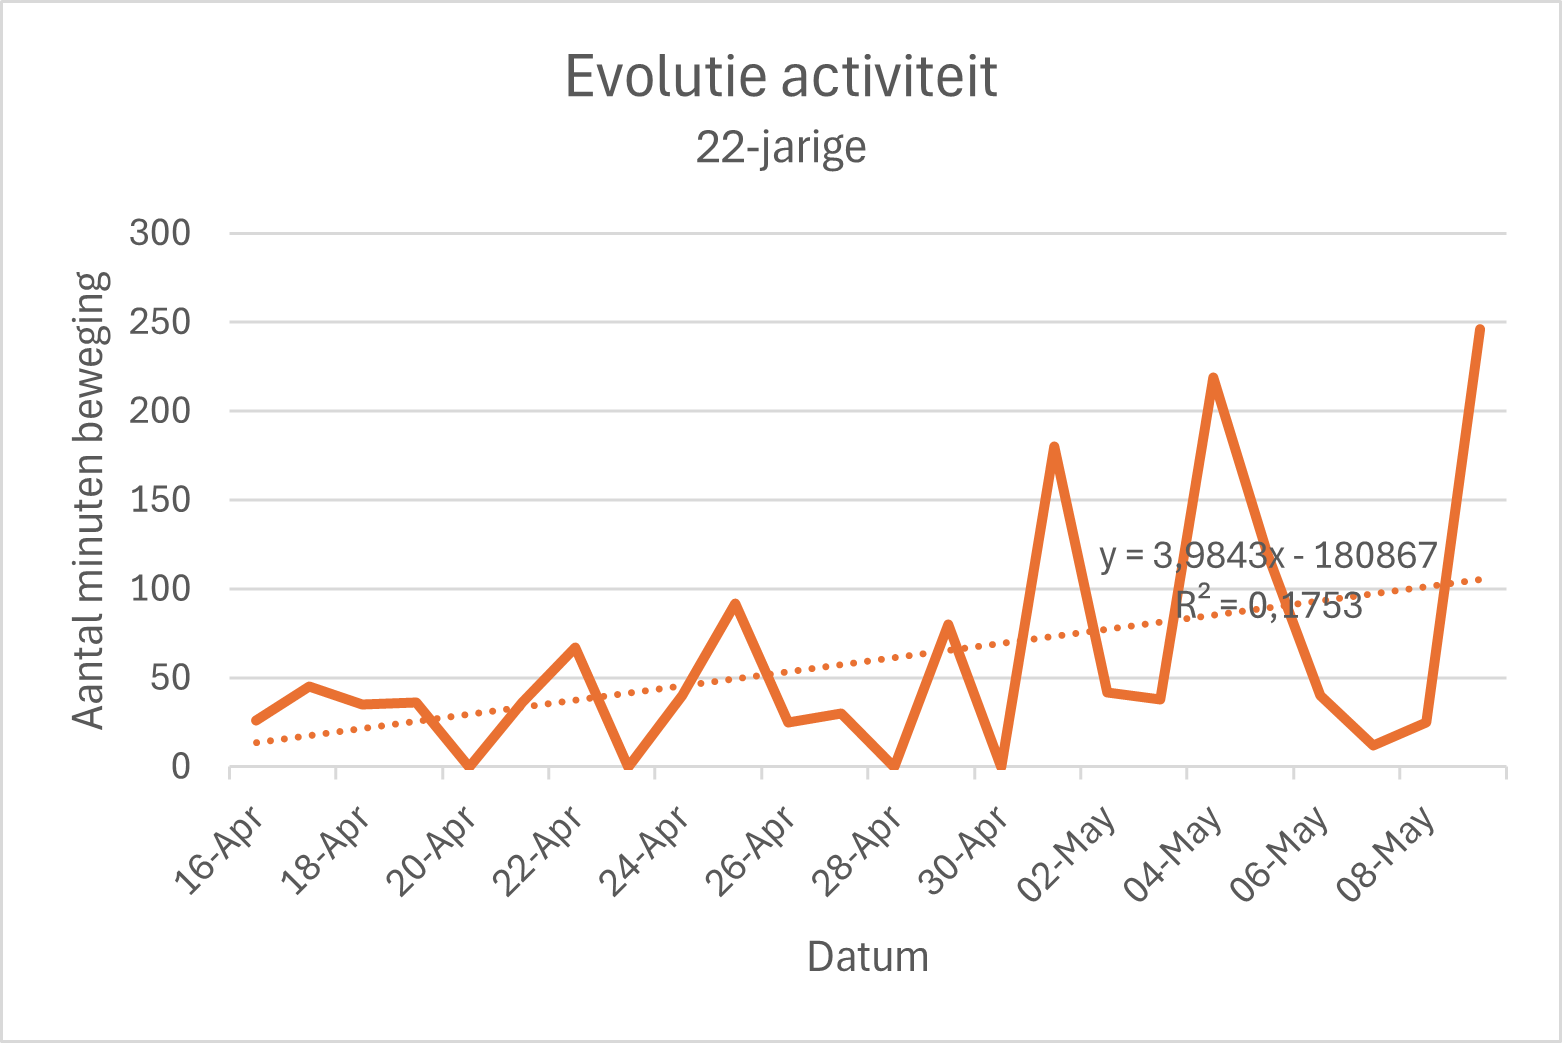
\includegraphics[width=1\textwidth]{GrafiekEvolutie2}
        \label{fig:evolutie2}
    \end{minipage}
\end{figure}

\begin{figure}[htbp]
    \begin{minipage}[t]{0.48\linewidth} % adjust width as needed
        \centering
        \caption[Evolutie van de activiteit van een 25-jarige]{Evolutie van de activiteit ingegeven in ``Move-it!'' van een 25-jarige.}
        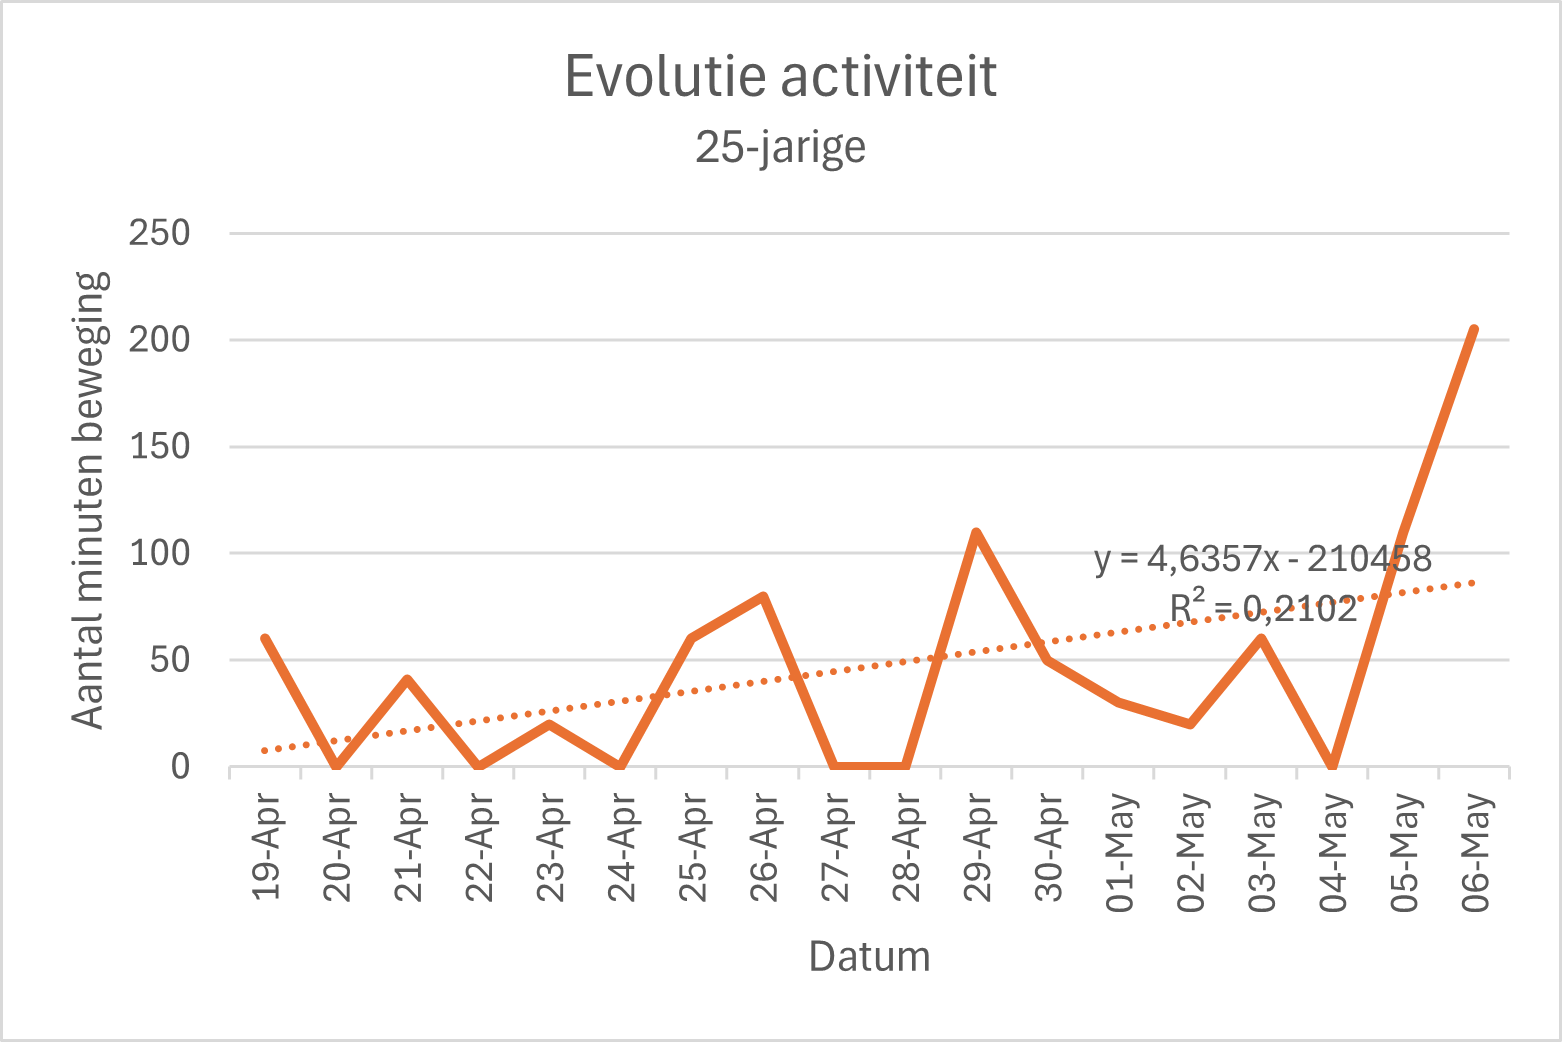
\includegraphics[width=1\textwidth]{GrafiekEvolutie3}
        \label{fig:evolutie3}
    \end{minipage}
    \hfill
    \begin{minipage}[t]{0.48\linewidth} % adjust width as needed
        \centering
        \caption[Evolutie van de activiteit van een 28-jarige]{Evolutie van de activiteit ingegeven in ``Move-it!'' van een 28-jarige.}
        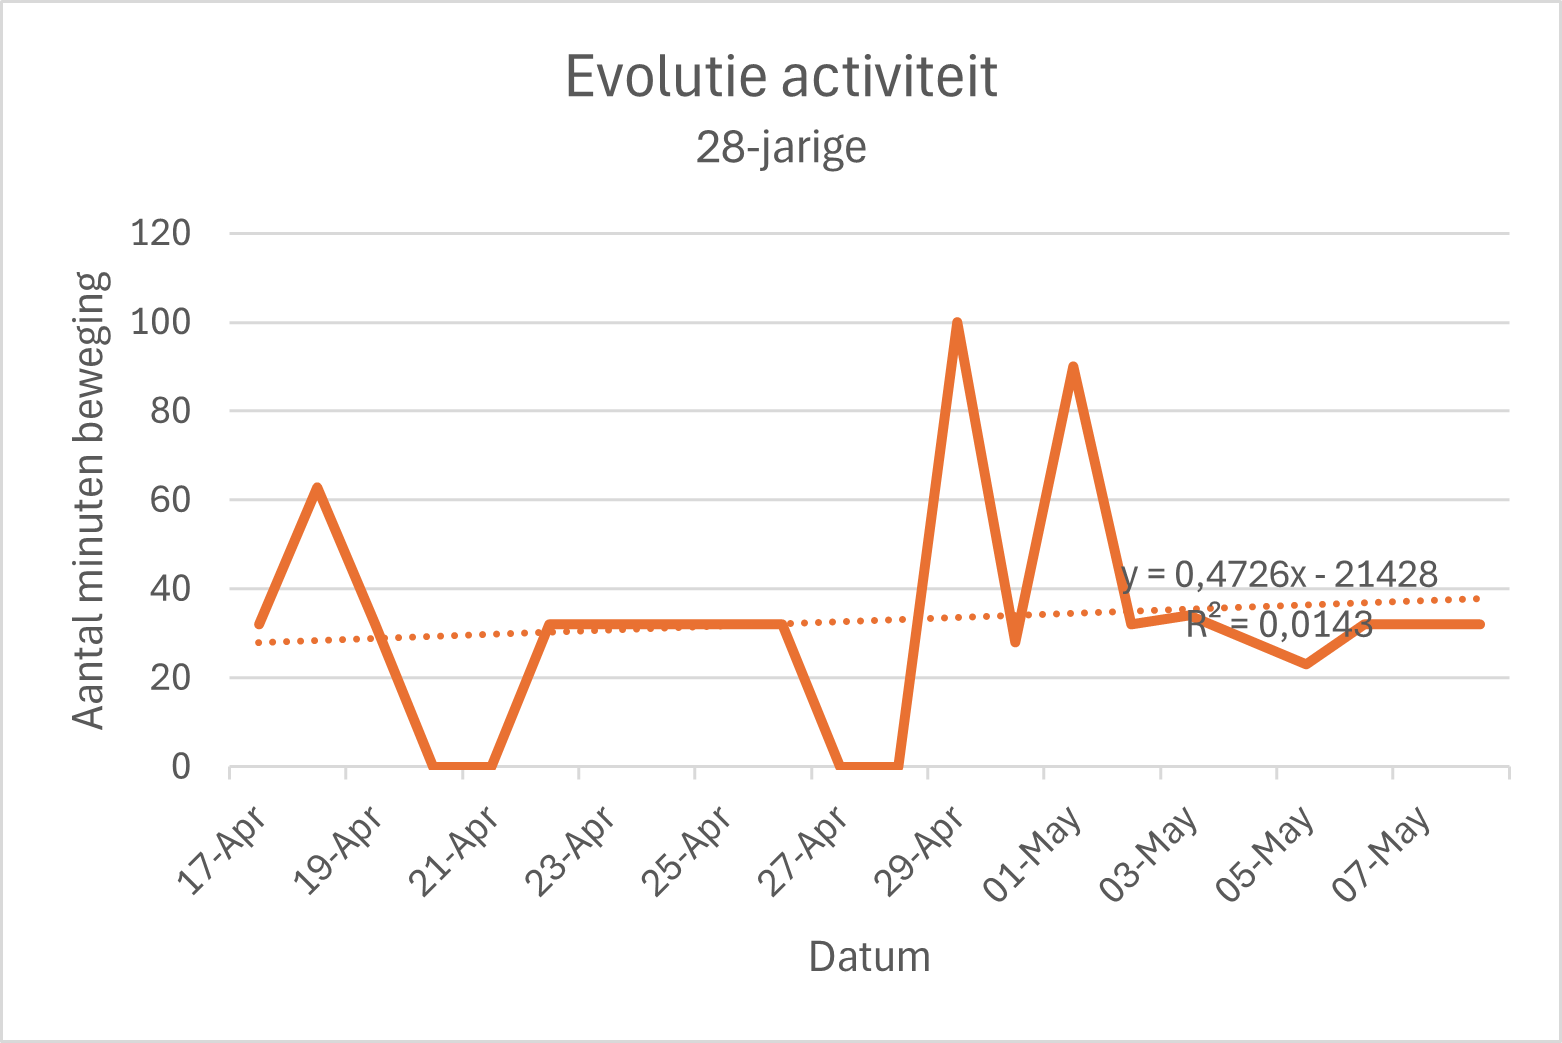
\includegraphics[width=1\textwidth]{GrafiekEvolutie4}
        \label{fig:evolutie4}
    \end{minipage}
\end{figure}
\begin{figure}[htbp]
    \begin{minipage}[t]{0.48\linewidth} % adjust width as needed
        \centering
        \caption[Evolutie van de activiteit van een 25-jarige]{Evolutie van de activiteit ingegeven in ``Move-it!'' van een 25-jarige.}
        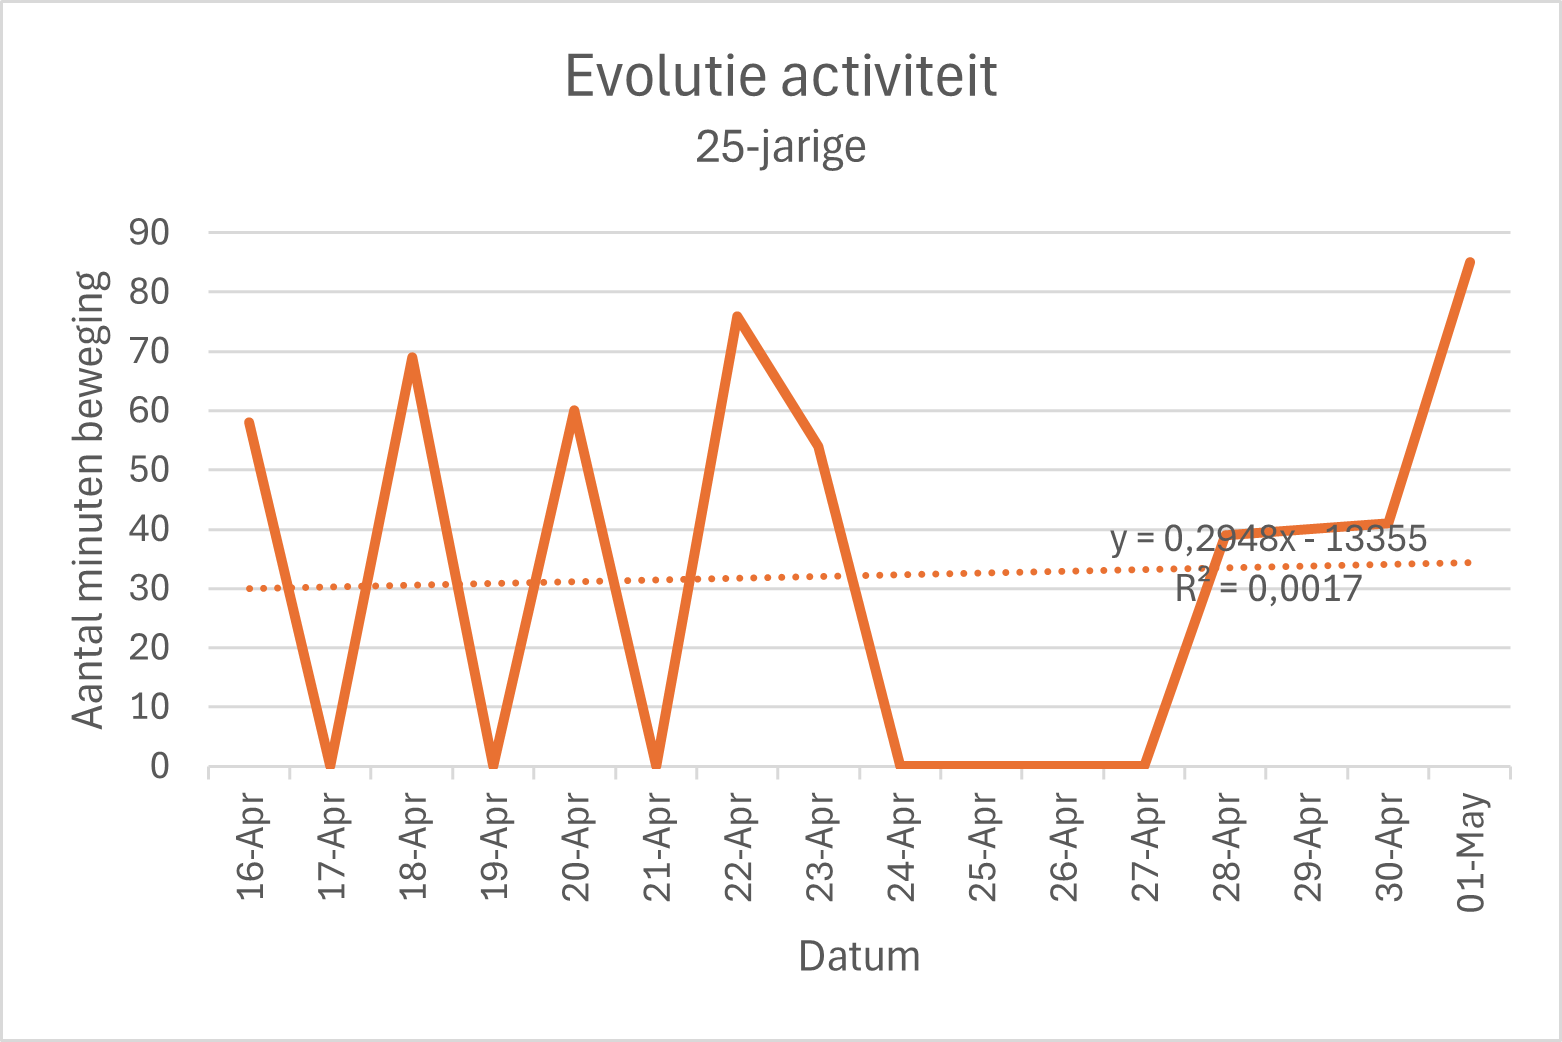
\includegraphics[width=1\textwidth]{GrafiekEvolutie5}
        \label{fig:evolutie5}
    \end{minipage}
    \hfill
    \begin{minipage}[t]{0.48\linewidth} % adjust width as needed
        \centering
        \caption[Evolutie van de activiteit van een 27-jarige]{Evolutie van de activiteit ingegeven in ``Move-it!'' van een 27-jarige.}
        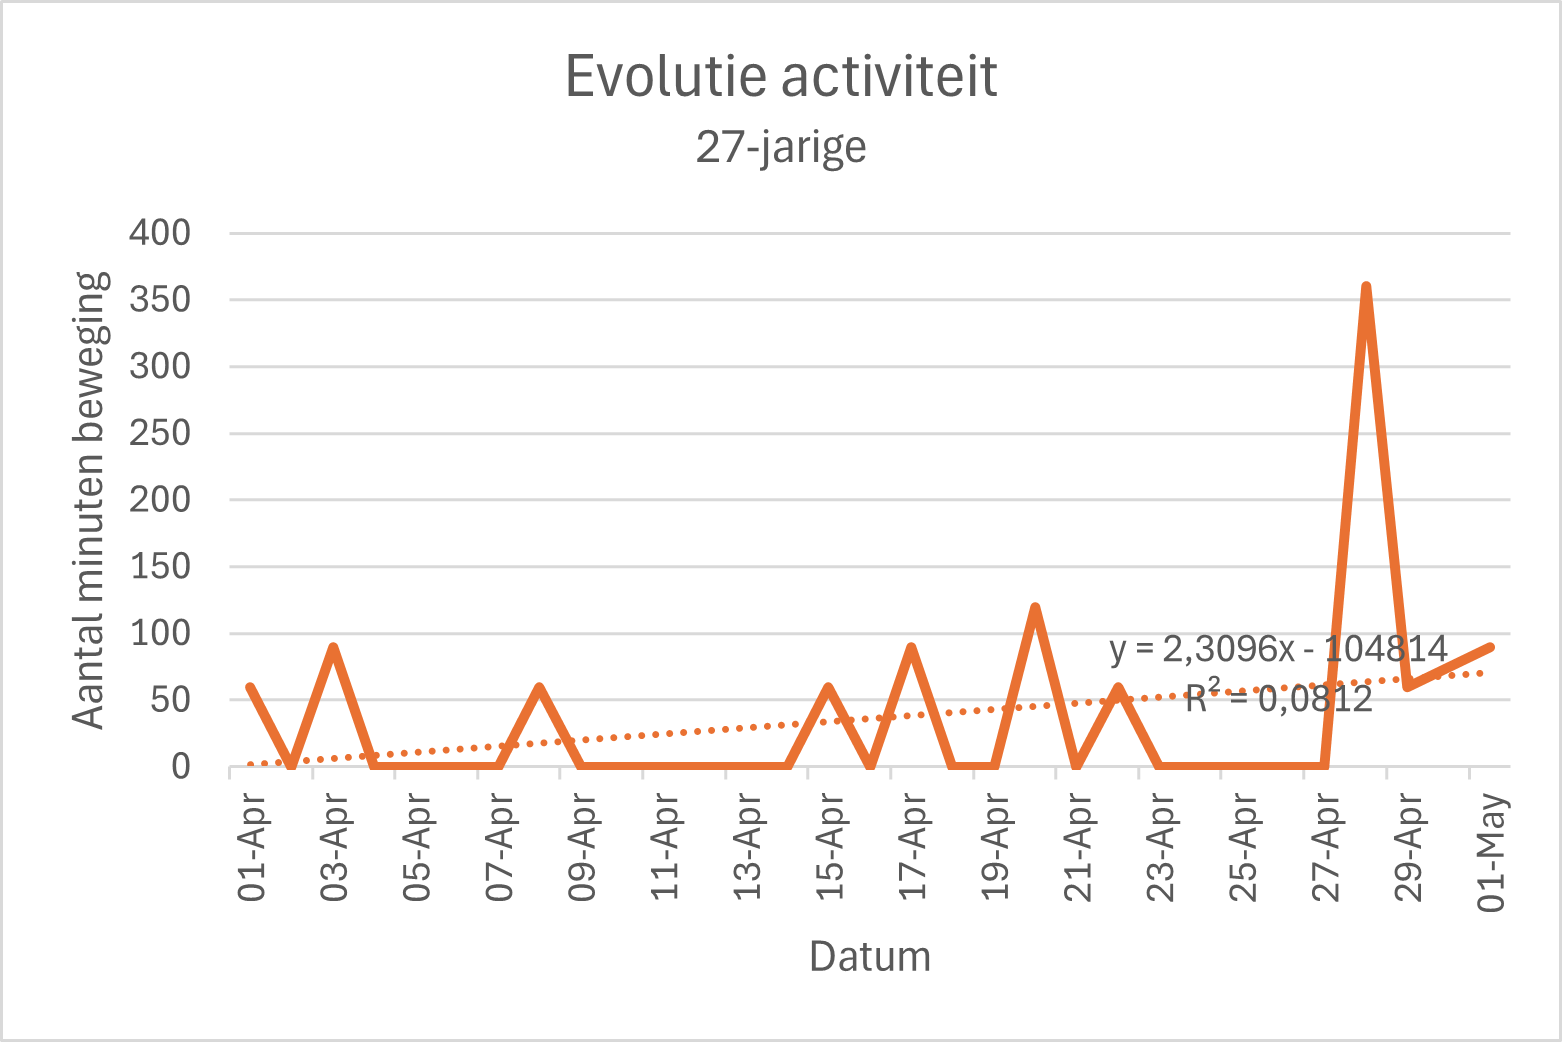
\includegraphics[width=1\textwidth]{GrafiekEvolutie6}
        \label{fig:evolutie6}
    \end{minipage}
\end{figure}
\begin{figure}[htbp]
    \begin{minipage}[t]{0.48\linewidth} % adjust width as needed
        \centering
        \caption[Evolutie van de activiteit van een 28-jarige]{Evolutie van de activiteit ingegeven in ``Move-it!'' van een 28-jarige.}
        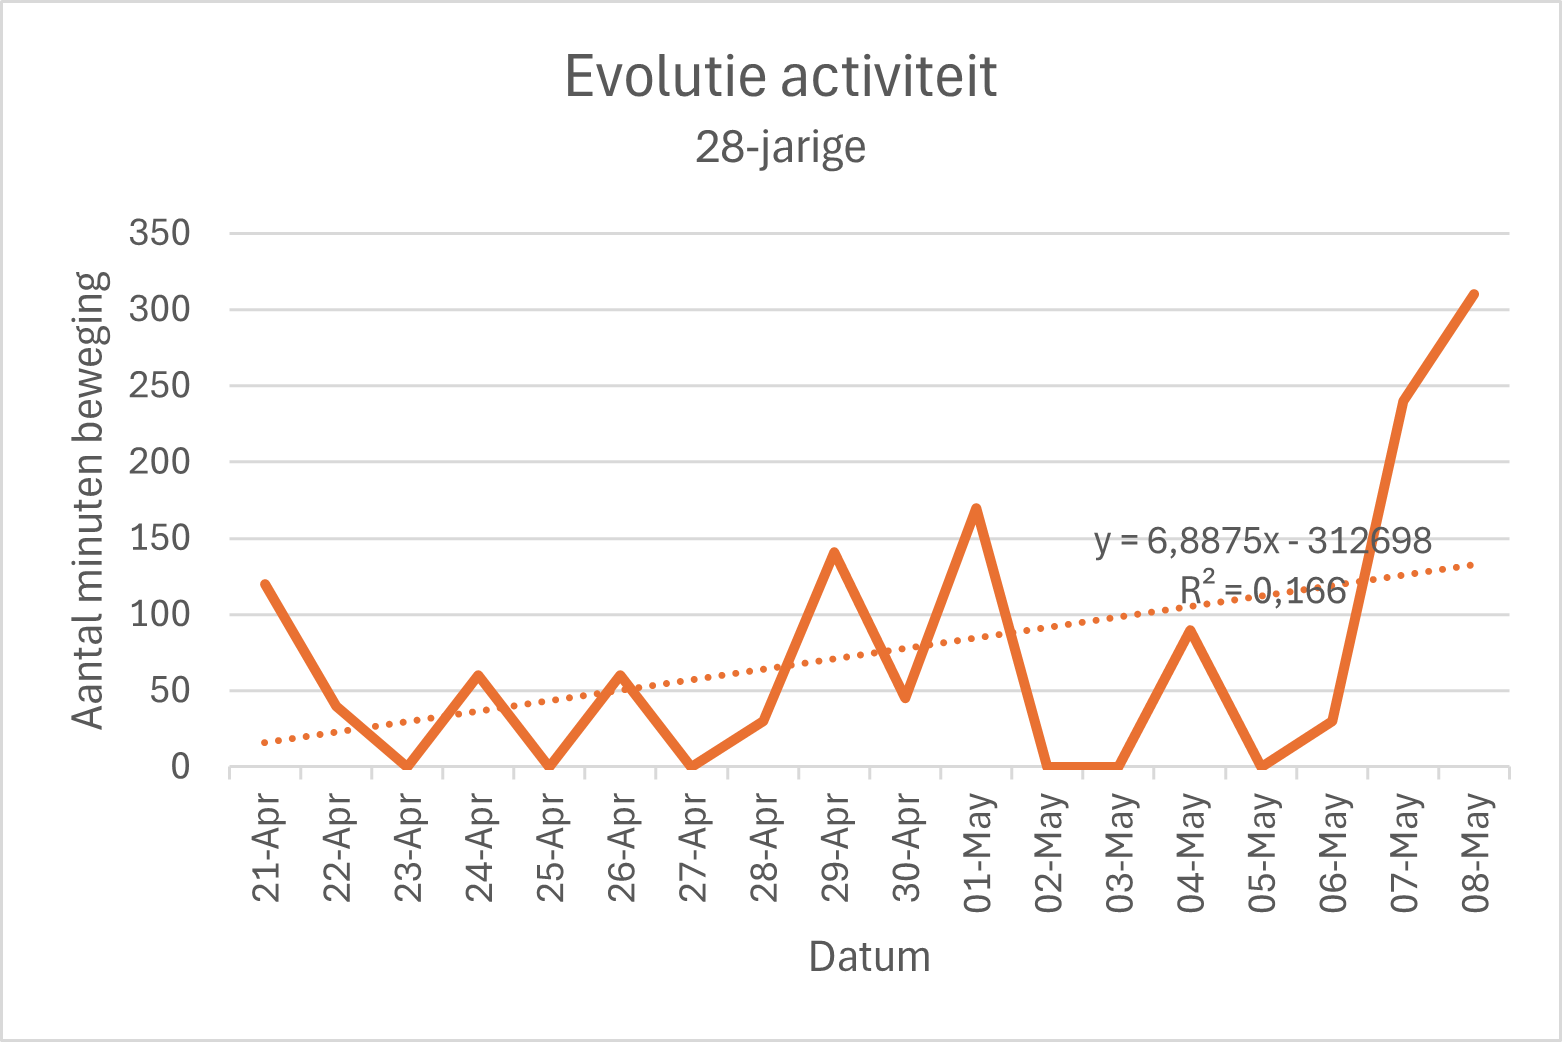
\includegraphics[width=.9\textwidth]{GrafiekEvolutie7}
        \label{fig:evolutie7}
    \end{minipage}
    \hfill
    \begin{minipage}[t]{0.48\linewidth} % adjust width as needed
        \centering
        \caption[Evolutie van de activiteit van een 22-jarige]{Evolutie van de activiteit ingegeven in ``Move-it!'' van een 22-jarige.}
        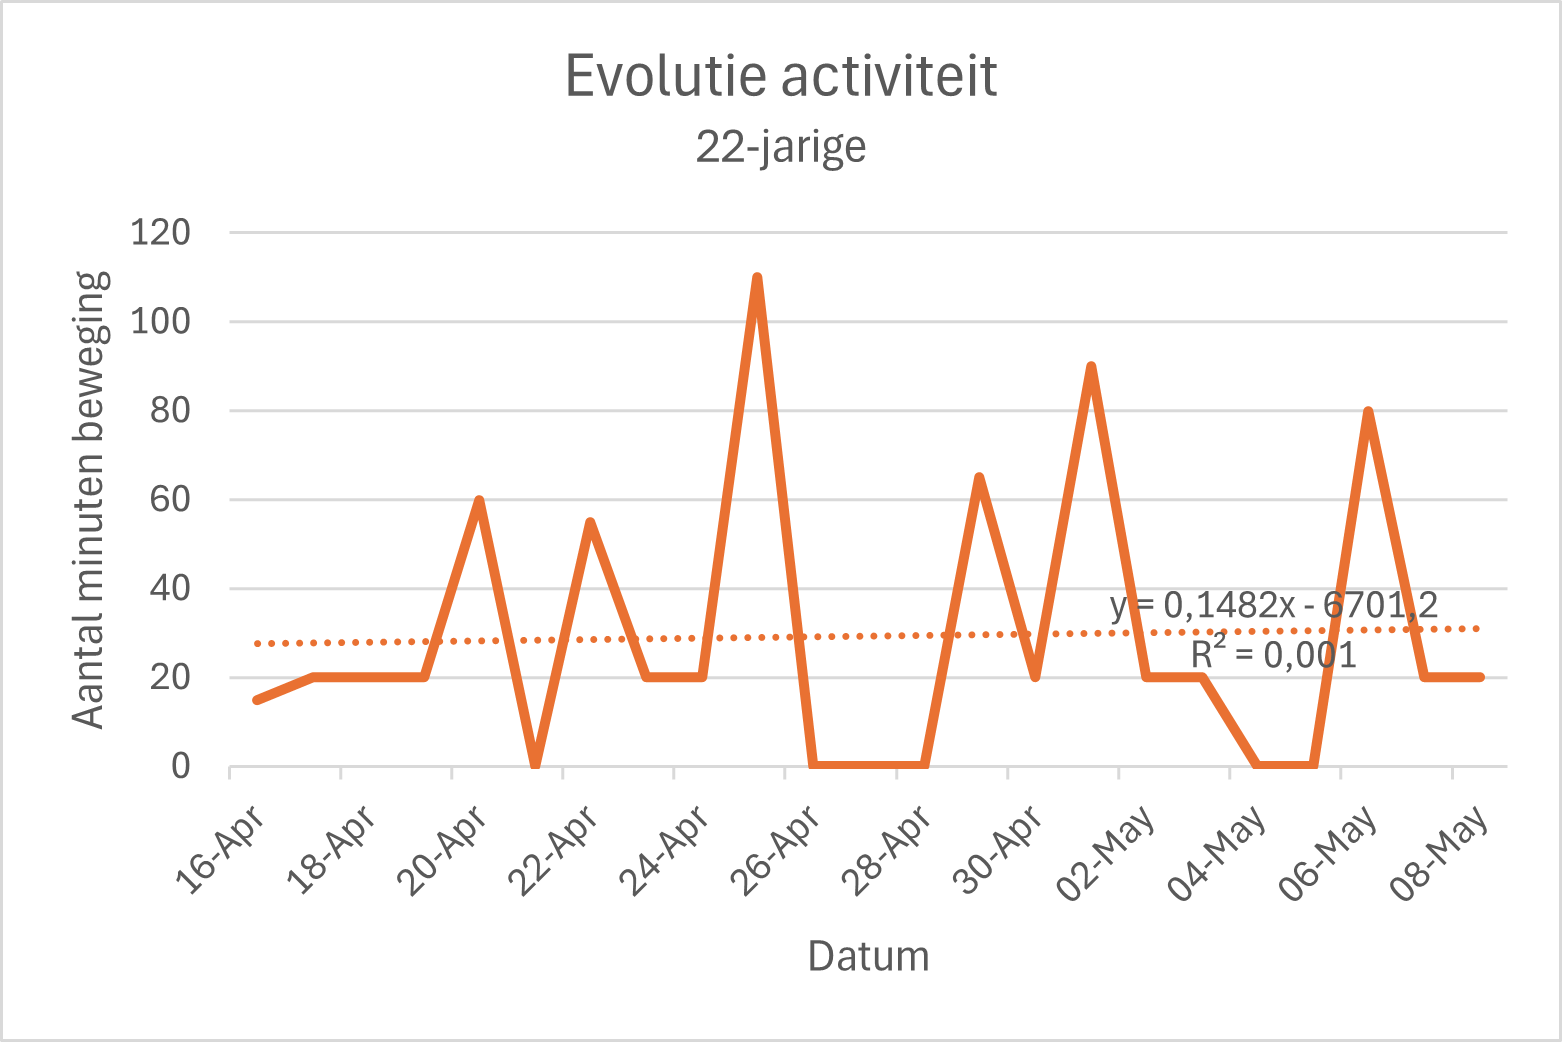
\includegraphics[width=.9\textwidth]{GrafiekEvolutie8}
        \label{fig:evolutie8}
    \end{minipage}
\end{figure}

Daarnaast kan uit de sportgegevens ook het gemiddeld aantal minuten beweging per dag en per week gehaald worden, met als doel te analyseren of de stijging in de hoeveelheid dagdagelijkse beweging zich heeft doorgezet tot het aangeraden niveau van de WHO. Hiervoor worden opnieuw de gegevens gebruikt van de acht proefpersonen waarvoor grafieken gegenereerd werden.

\begin{table}[h]
    \caption[Gemiddeld aantal minuten beweging per dag en per week]{Gemiddeld aantal minuten beweging per dag en per week van de meest consistente deelnemers.}
    \centering
    \label{table:gemiddeldes}
\begin{tabular}{||m{.2\linewidth} m{.4\linewidth} m{.4\linewidth}||}
    \hline
    Leeftijd & Gemiddeld aantal minuten beweging per dag & Gemiddeld aantal minuten beweging per week \\ [0.5ex]
    \hline\hline
    22 & 59.75 & 418.25 \\
    22 & 29.35 & 205.45 \\
    25 & 47 & 329 \\
    25 & 32.13 & 224.91 \\
    27 & 63.96 & 447.72 \\
    27 & 35 & 245 \\
    28 & 32.86 & 230.02 \\
    28 & 74.22 & 519.54 \\ [1ex]
    \hline
\end{tabular}
\end{table}

De cijfers uit tabel \ref{table:gemiddeldes} geven het gemiddeld aantal minuten beweging per dag en per week terug, berekend op basis van de data die gedurende vier weken verzameld is.
Deze suggereren dat jongeren tussen de 22 en 28 jaar de vooropgestelde bewegingsnormen van de WHO wel degelijk behalen.
Het is daarbij wel zeer belangrijk te vermelden dat dit onderzoek geen onderscheid kan maken tussen sportieve activiteiten met gemiddelde of intensieve inzet. Daarom ziet het de bekomen data als de som van de gemiddeld intense en erg intensieve activiteiten. Als minimum wordt daarom ook de som genomen, wat neerkomt op 225 à 450 minuten per week. Dit specifiek aspect moet verder besproken worden in een onderzoek waarin elke proefpersoon een hartslagmonitor ter beschikking krijgt, waardoor een onderscheid zal kunnen gemaakt worden tussen beide types activiteiten.

Tenslotte moet volgende bemerking gemaakt worden: geven deelnemers die uit zichzelf regelmatig intensief sporten niet al hun bewegingsgegevens in of bewegen ze effectief weinig daarnaast? Het kan bijvoorbeeld zo zijn dat zeer fitte mensen woon-werkverkeer niet beschouwen als ``echt'' bewegen, omdat hun lichaam een veel hogere intensiteit gewoon is. Dit is nog een vraag die uitnodigt naar verder onderzoek.

\section{Resultaten na gebruik van ``Move-it!''}

\subsection{Beweging}

% TODO: echte cijfers aanpassen

Voor aanvang van het gebruik van ``Move-it!'', gaf 81\% van de deelnemers aan meer te willen sporten. Na het in gebruik nemen van het sportplatform, is dit gedaald naar 63.6\%.
45.5\% van de deelnemers geeft ook aan tevreden te zijn met diens dagelijkse beweging. Daarbovenop geven 54.6\% van de deelnemers aan dat ze meer dan 150 minuten per week bewegen met gemiddelde intensiteit, wat een lichte stijging is ten opzichte van de 47.5\% voordien. Voor sporten met hoge intensiteit,

Uit de sportgegevens kan afgeleid worden dat deelnemers over het algemeen wel degelijk meer bewegen sinds het gebruiken van de applicatie. Dit komt ook terug uit de vragenlijst, waarin 54.5\% aangeeft het gevoel te hebben meer te bewegen sinds het in gebruik nemen van ``Move-it!''.

Wanneer bevraagd wordt hoe een sportapplicatie kan helpen om meer te bewegen, kwamen volgende zaken aan bod:

\begin{itemize}
    \item Een trainingsschema voorzien.
    \item Inspiratie bieden op vlak van oefeningen of soorten bewegen, om zo variatie te brengen.
    \item Een sociaal gebeuren creëren, om zo gelijk gezinde mensen te vinden.
    \item Een realistische en flexibele planning kunnen opstellen, aangepast aan de eigen (soms zeer drukke) agenda, waarin trainingen verplaatst kunnen worden.
\end{itemize}

Tenslotte geeft 50\% aan het gevoel te hebben productiever te zijn sinds het gebruik van de sportapplicatie. De overige 50\% heeft hier geen mening over.

\subsection{Motivatie}

% TODO: echte cijfers aanpassen
% TODO: verwijzen naar literatuur voor competitiviteit
Bij het in gebruik nemen van het sportplatform, viel het op dat niet iedereen even consistent was met het ingeven van data. Een mogelijke oorzaak hiervan zou te vinden zijn bij de competitiviteit van de deelnemers. Uit de bevraging op het einde van de testperiode van ``Move-it!'', is gebleken dat van alle deelnemers 9.1\% niet en 9.1\% slechts een beetje competitief ingesteld is. Dit verklaart vermoedelijk een deel van de inconsistentie waarmee sommigen gegevens ingaven.
Een andere mogelijke oorzaak hiervoor zou ook het manueel ingeven van de gegevens kunnen zijn, gezien dit ook enkele keren terugkwam in de suggesties om het platform beter te maken (zie ook \ref{ssec:verbeterpunten}).

\subsection{Gamification}

Het populairste deel van de gamification, is de persoonlijke ranking: 81.8\% van de deelnemers geeft aan dit als motiverend te ervaren. Daarna volgen het opvolgen van de eigen vooruitgang, door middel van de grafieken op het dashboard en door middel van de tabel op het persoonlijk overzicht, beiden met 54.5\%. Op de laatste plaats staat de lijst van de eigen gepresteerde activiteiten et 36.4\%.

\subsection{Verbeterpunten sportplatform}
\label{ssec:verbeterpunten}

Tijdens de laatste bevraging werd er ook ruimte gelaten voor suggesties om het sportplatform nog te verbeteren, hierbij geeft 54.5\% aan dat een bepaalde verandering er voor zou kunnen zorgen dat desbetreffende deelnemer het sportplatform vaker zou gebruiken. De meest voorkomende verbeterpunten zijn:

\begin{itemize}
  \item Het mogelijk maken om sportprestaties te bewerken.
  \item Het makkelijker maken om sportgegevens in te geven, door bijvoorbeeld integratie met Strava.
  \item Scores bepalen aan de hand van de intensiteit van de activiteiten.
\end{itemize}